
The thermo-electrical model provides a wide range of predictions for the operation of the strip system. A detailed discussion of all results is beyond the scope of this article; instead, we present here a subset of the results to demonstrate the capabilities and use of the thermo-electrical model for the design of the detector system.

\subsection{Operational scenarios}\label{sec:opscenarios}
To study the different aspects of our predictions for the operation of the ITk strip system throughout its lifetime, we performed the calculation of the system parameters over the expected 14 years of operation in monthly steps as outlined in Section~\ref{sec:running}. Time-dependent operational inputs to the calculation were taken from the expected performance of the HL-LHC (Fig.~\ref{fig:lhc_profile}). For the cooling, which can be adjusted during data taking using detector control systems, we studied flat (constant) coolant temperature profiles ranging from from $0^\circ$C to $-35^\circ$C, the lowest evaporation temperature achievable with the ITk evaporative CO$_2$ cooling system. We also studied a `ramp' scenario in which the coolant temperature starts at 0$^\circ$C and is gradually lowered down to $-35^\circ$C over the course of 10 years (Fig.~\ref{fig:coolant_ramp}).
% Consider adding above: The total ionizing dose rate (required to calculate the TID bump) and the NIEL fluence (used to determine the sensor leakage current) are calculated for each month using the information in Fig~\ref{fig:radiation} and Fig.~\ref{fig:lhc_profile}.

\begin{figure}[ht]
\centering
\subfloat[] {\label{fig:lhc_profile}  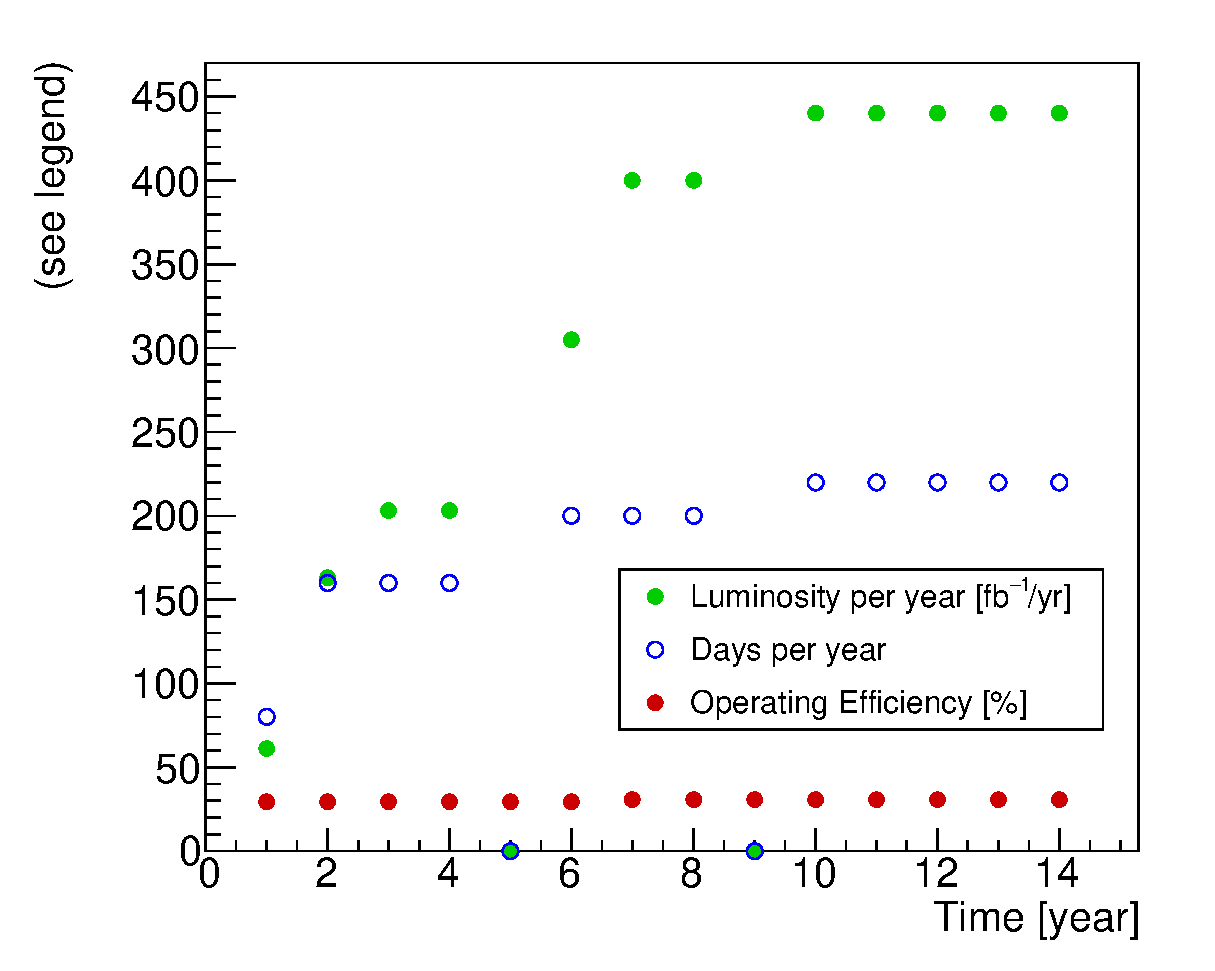
\includegraphics[width=0.45\linewidth]{figures/YearlyRunProfile.eps}}\quad\quad
\subfloat[] {\label{fig:coolant_ramp} 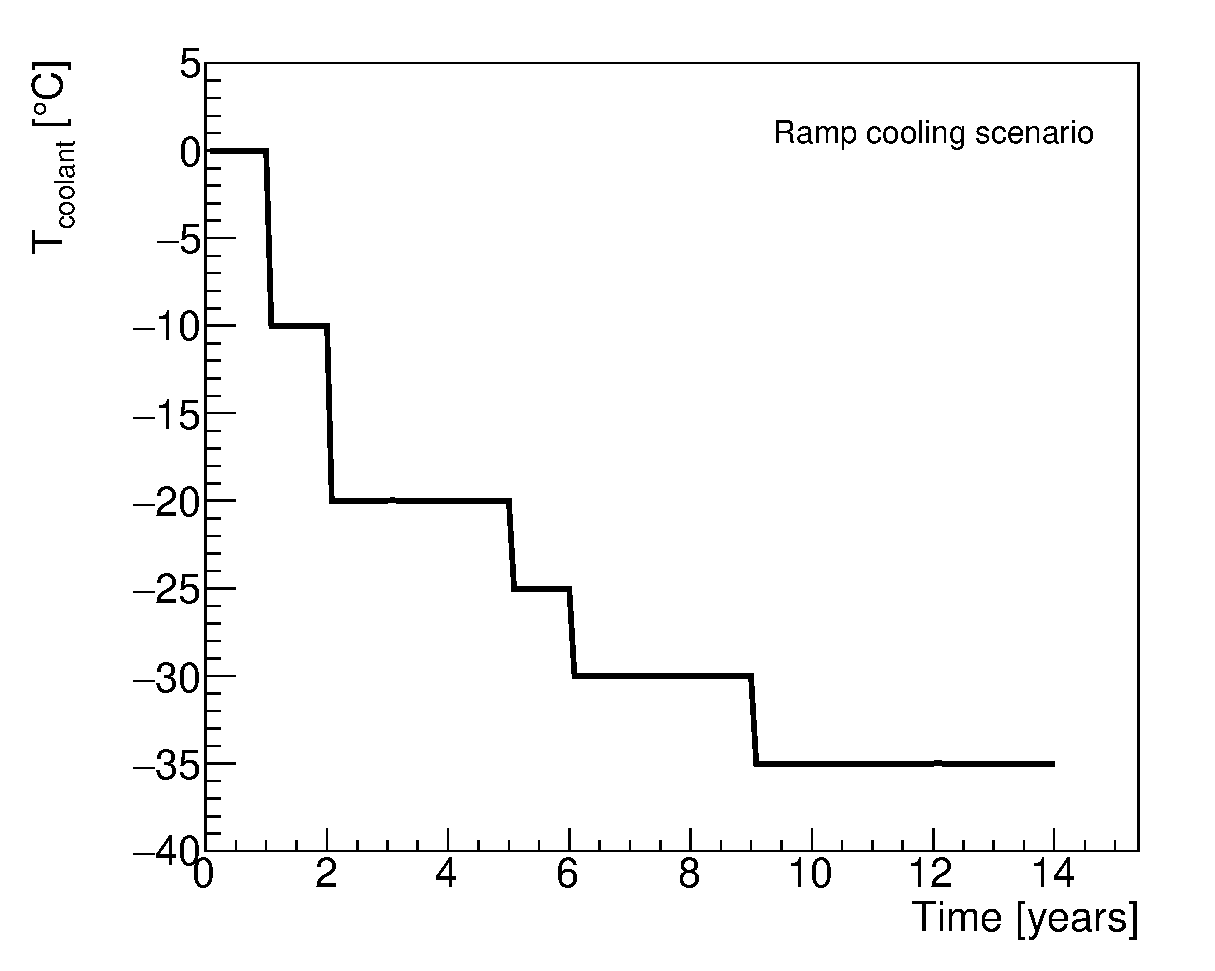
\includegraphics[width=0.45\linewidth]{figures/CoolantTemperature_RampScenario.eps}}
\caption{(a) Expected HL-LHC performance and (b) `cooling ramp' scenario for the coolant temperature. Year-long shutdowns of the LHC are anticipated in years 5 and 9.}
\label{fig:opscenarios}
\end{figure}

\subsection{Safety factors}
\label{sec:safety_factors}
To ensure the robustness of the system design against uncertainties in the assumptions used in the model, we also evaluate the model using a set of input parameters with some key inputs degraded. The set of safety factors used is given in Table~\ref{tab:safetyfactors}. Each safety factor has been estimated individually based on experience, the complexity of the system aspect described by the parameter, and from available data or the absence of such data. Note that the model can be evaluated with all the safety factors listed in Table~\ref{tab:safetyfactors} used together, a situation that is unlikely to occur in the real system, to provide a worst-case estimate for the performance of the ITk strip system. The individual effects of the different safety factors are demonstrated in Fig.~\ref{fig:safety_factors}.

\let\arraystretcha\arraystretch %% improve the table spacing
\renewcommand\arraystretch{1.2} %% improve the table spacing
\begin{table}[htb]
\caption{Safety factors.}
\label{tab:safetyfactors}
\centering
\adjustbox{max width=\textwidth}{ %% just before tabular
\begin{tabular}{lcl}
\toprule
Safety factor & Value & Reason \\
\midrule
\multirow{2}{*}{Fluence}  & \multirow{2}{*}{50\%} & Accuracy of fluence calculations and uncertainties\\
                          &                       & in material distributions\\
Thermal impedance & 10\% barrel, 20\% endcap & Local support build tolerances, thermal network assumptions\\
Digital current & 20\% & Final chip performance and parametrization of TID effect\\
Analog current & 5\% & Final chip performance\\
Tape electrical impedance & 10\% & Electrical tape manufacturing tolerances\\
Bias voltage & 700~V & Increased bias voltage from nominal 500~V to maintain S/N\\
TID parametrization & Nominal/Pessimistic & Different data sets for fit of TID bump\\
\bottomrule
\end{tabular}
} %% adjustbox after tabular
\end{table}
\let\arraystretch\arraystretcha %% reset the table spacing

\begin{figure}[ht]
\centering
\subfloat[] {\label{fig:safety_factors_a} 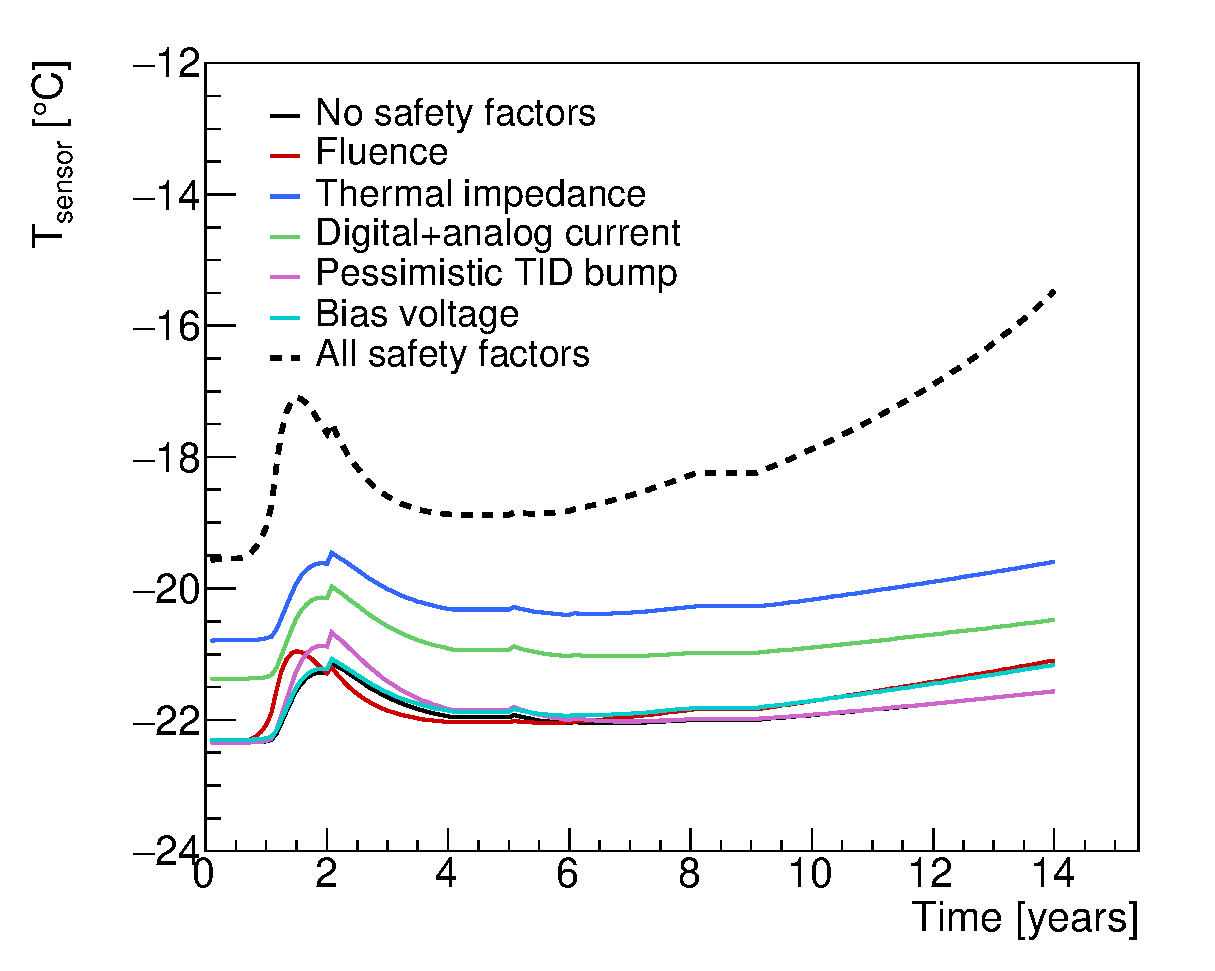
\includegraphics[width=0.45\linewidth]{figures/CompareSafetyFactors_SensorTemperature_R3.eps}}\quad\quad
\subfloat[] {\label{fig:safety_factors_b} 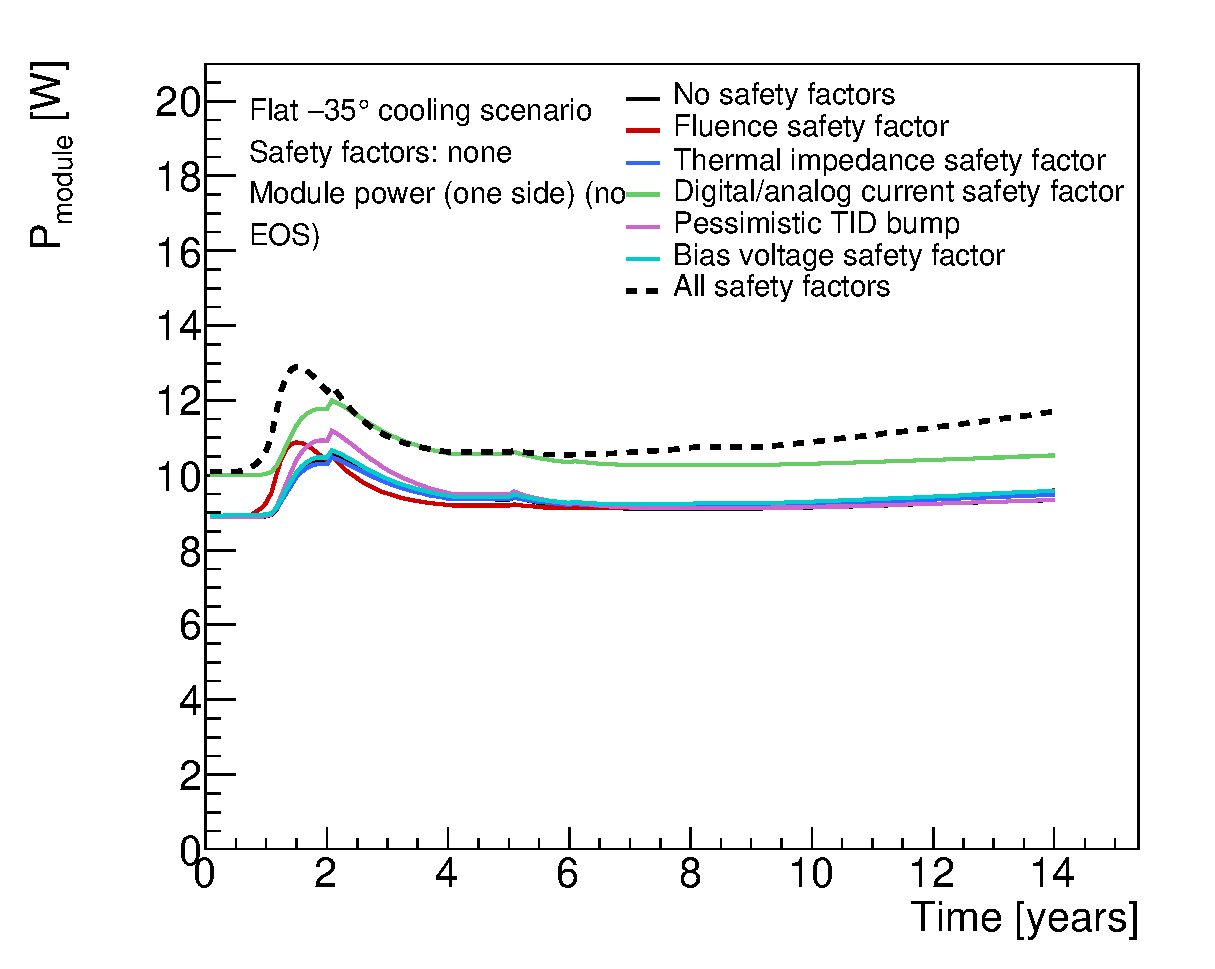
\includegraphics[width=0.45\linewidth]{figures/CompareSafetyFactors_ModulePower_R3.eps}}
\caption{Comparing the impact of different safety factors on (a) the sensor temperature and
(b) the module power for the endcap R3-type module, using a flat cooling scenario ($-30^\circ$C). The dotted line depicts the effect of all safety
factors applied at once.}
\label{fig:safety_factors}
\end{figure}

It is important to note that combining multiple safety factors can have a compounding effect on the system. As an example, the effect of an increased bias voltage combined with a larger digital current will result in a much higher sensor leakage current at the detector end-of-life than either situation occurring individually. The analytical model presented here allows for scenarios like these to be examined quickly and effectively.

\subsection{Module properties}

Several module properties predicted by the thermo-electrical model are shown in Figs.~\ref{fig:moduleflatperformance} and~\ref{fig:modulerampperformance} for the barrel system. The different radiation-dependent effects occur on different timescales. The maximum in the digital chip power due to the TID effect occurs relatively early (in year 1 to 4), although the bump has a long tail, particularly in the outer layers of the barrel. The sensor leakage power, on the other hand, grows towards the end of the lifetime of the ITk. If the leakage current continued to increase in the case of further irradiation, or if the cooling temperature were raised, this growth would ultimately lead to thermal runaway. Due to the radial dependence of the radiation environment, the radiation-induced effects are most pronounced in the innermost barrel layers.

\begin{figure}[ht]
\centering
\subfloat[] {\label{fig:moduleflatperformance_a} 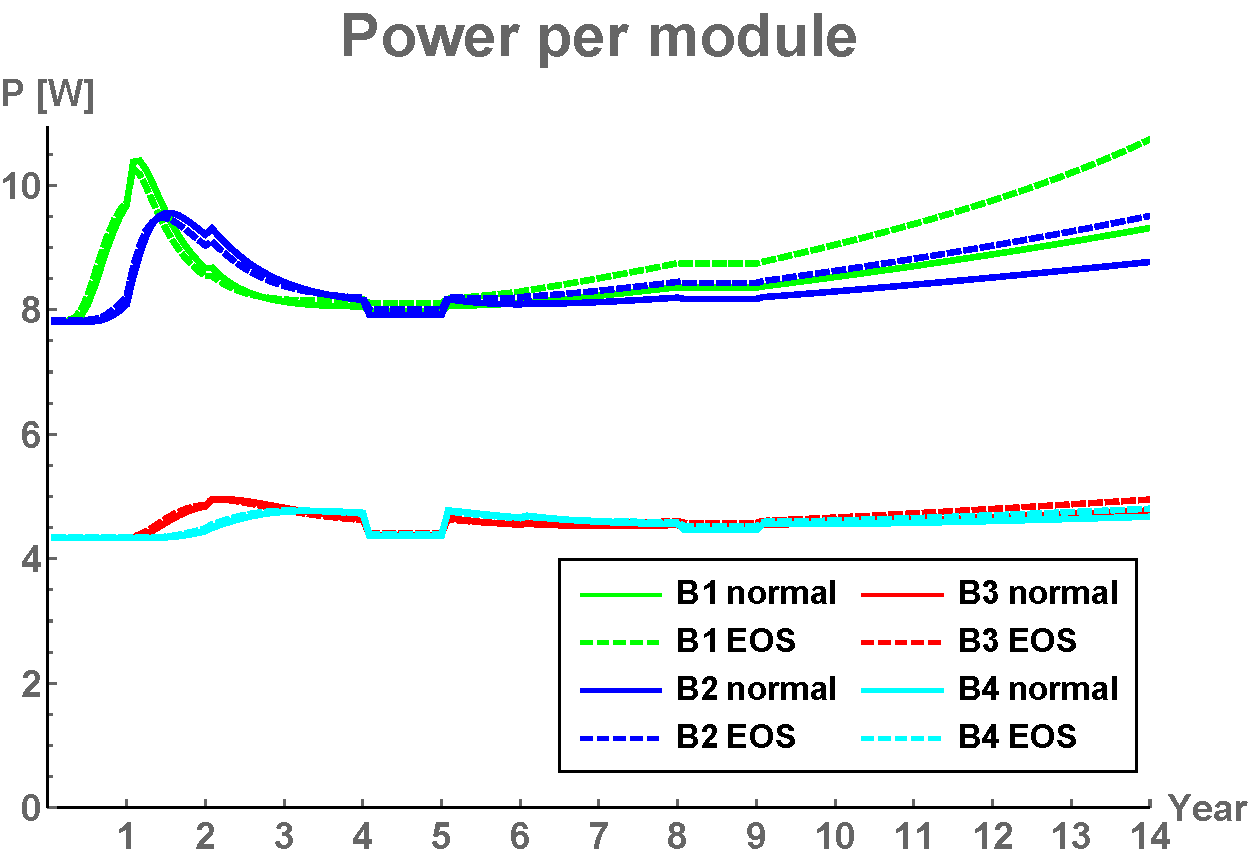
\includegraphics[width=0.45\linewidth]{figures/powerpermodule.pdf}}\quad\quad
\subfloat[] {\label{fig:moduleflatperformance_b} 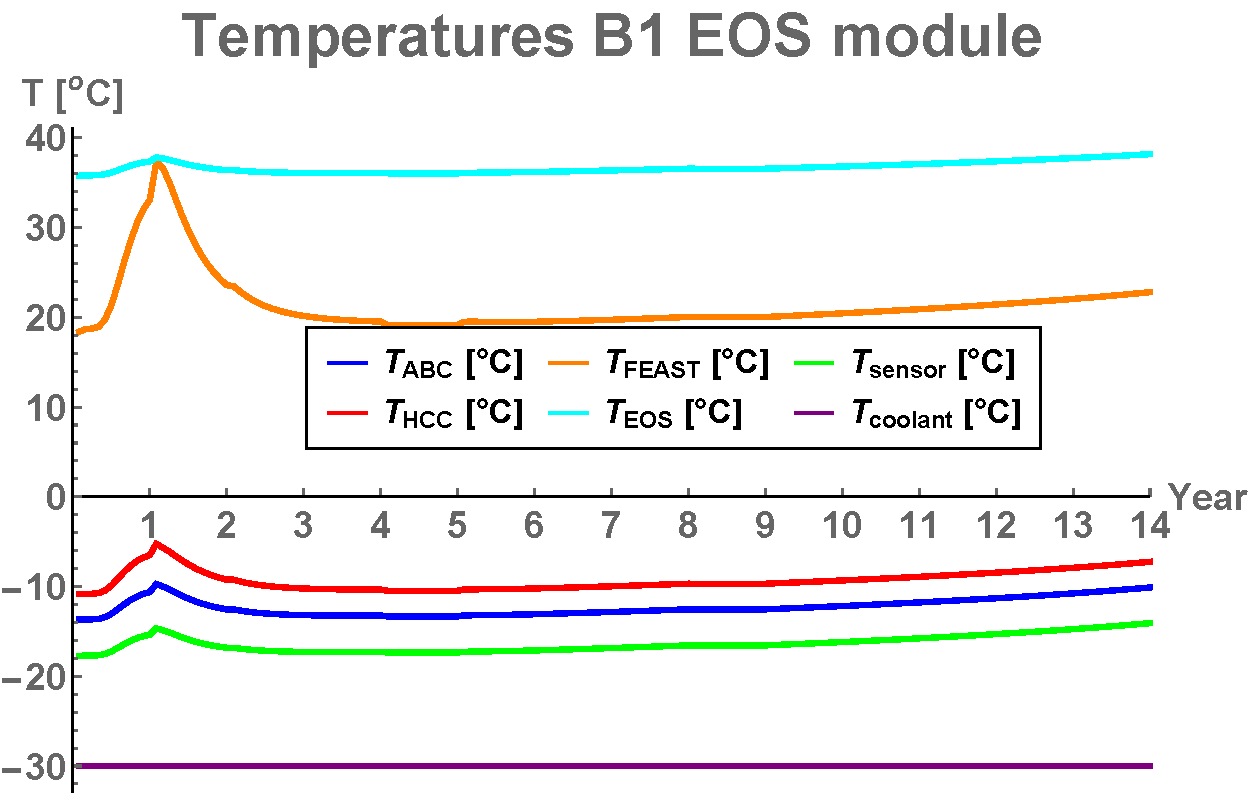
\includegraphics[width=0.45\linewidth]{figures/Teosmodule.pdf}}
\caption{Examples of barrel module performance predictions for a flat cooling scenario ($-30^\circ$C) including safety factors. (a) Power per module. (b) Temperatures for different nodes of an end-of-stave barrel module in the innermost barrel. The discontinuities in year 5 and 9 are due to anticipated year-long shutdowns of the LHC.}
\label{fig:moduleflatperformance}
\end{figure}

\begin{figure}[ht]
\centering
\subfloat[] {\label{fig:modulerampperformance_a} 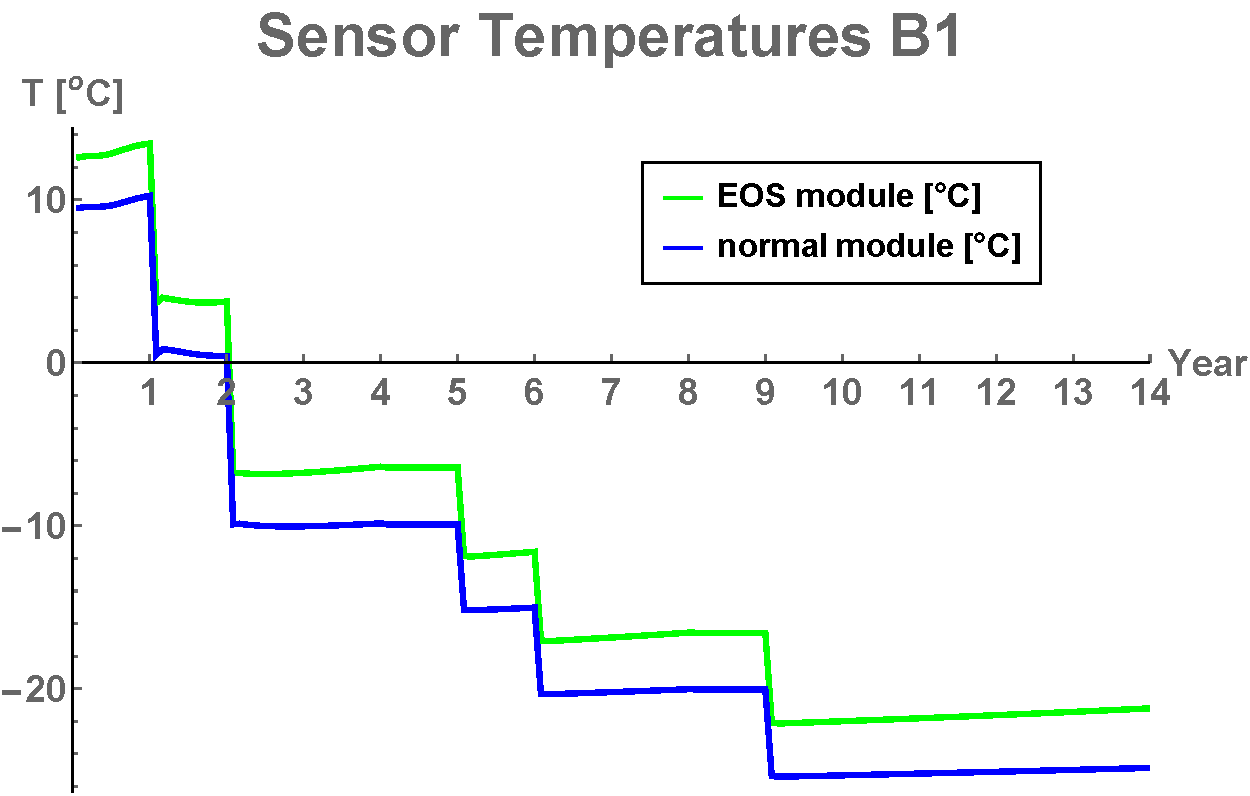
\includegraphics[width=0.45\linewidth]{figures/Tmodule.pdf}}\quad\quad
\subfloat[] {\label{fig:modulerampperformance_b} 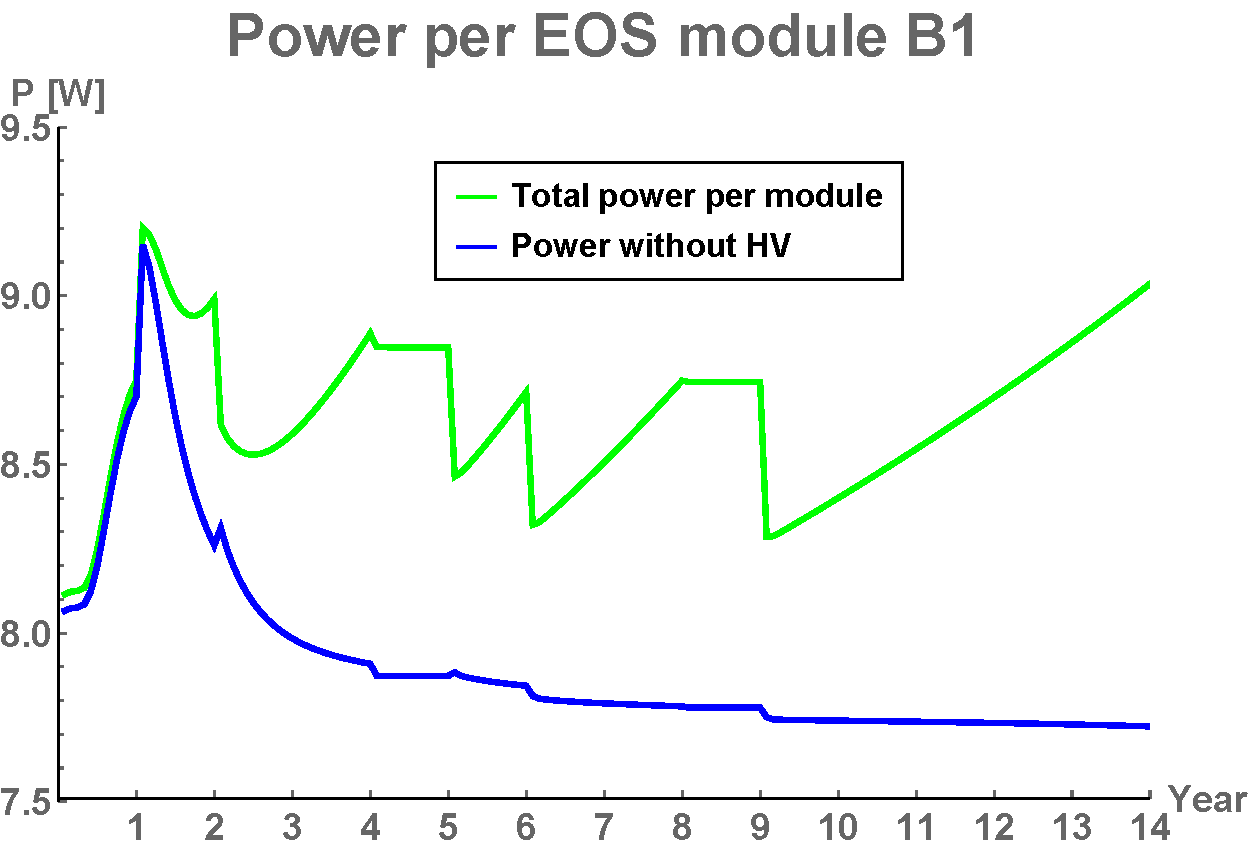
\includegraphics[width=0.45\linewidth]{figures/Peosmodule.pdf}}
\caption{Examples of barrel module performance predictions for the ramp cooling scenario including safety factors. (a) Sensor temperature in the innermost barrel modules. (b) Power in an end-of-stave barrel module in the innermost layer.}
\label{fig:modulerampperformance}
\end{figure}

\subsection{System properties}\label{sec:systemprop}
One of the key concerns for the design of the strip system is thermal stability of the system. If the cooling temperature is too high to limit the leakage power from the radiation-damaged sensors to a level where the heat can still be removed, the system is unstable (it goes into `thermal runaway').
% In this case, there is no solution to the set of equations in the thermo-electrical model anymore, and the numerical search for a solution fails.
% In the barrel strip system, this occurs in the final year of operation at a cooling temperature of $-15^\circ$C under nominal conditions, and at $-25^\circ$C (in year 13) with safety factors applied.
To find the cooling temperature $T_\text{C}$ at which this condition is reached, we make repeated simulations of the ITk strip system using the thermo-electrical model, with each simulation representing the full 14-year operation of the ITk at a fixed $T_\text{C}$. Between simulations, $T_\text{C}$ is increased in steps of 5$^\circ$C until the model finds thermal runaway. In the numeric evaluation of the thermo-electrical model this manifests itself in the absence of a solution to the system of equations. In the endcap strip system, this occurs at a cooling temperature of $-15^\circ$C under nominal conditions (i.e. with no safety factors applied); in this scenario, thermal runaway would be reached in the 12$^\text{th}$ year of operation. With all safety factors applied, thermal runaway would occur at a cooling temperature of $-25^\circ$C (in year 10).
In the barrel system, where the radiation environment is slightly less intense, the conditions for thermal runaway occur at the same cooling temperatures, but a few years later than in the endcaps: in the final year of operation and a cooling temperature of $-15^\circ$C under nominal conditions, and at $-25^\circ$C (in year 13) with safety factors applied.
As the design cooling temperature of the ITk cooling system is $-35^\circ$C, we have confidence that the ITk strip system has a sufficient margin for thermal stability.

Beyond the issue of stability, the thermo-electrical model delivers predictions for the development of current and power requirements for the overall system. Some of the predictions are shown in Fig.~\ref{fig:systemperformance}. Again, the different timescales of the various radiation-induced effects are visible; ignoring this time dependence could lead to over-specification of some system aspects.
Taking Fig.~\ref{fig:systemperformance_b} as an example, the average module power (indicated by the thick black line) is 6.6~W in the beginning of operation and reaches 8.0~W at the TID bump, in the second year. If we naively summed the maxima of the TID bumps, neglecting time dependence, we would arrive at 8.6~W, overestimating the power at the TID bump by 7.5\% and overestimating the effect of the TID bump by 43\%.
The difference, multiplied in the endcap by 4608 modules, amounts to nearly 3~kW of power and impacts the specifications of e.g. the cooling system.

\begin{figure}[ht]
\centering
\subfloat[] {\label{fig:systemperformance_a} 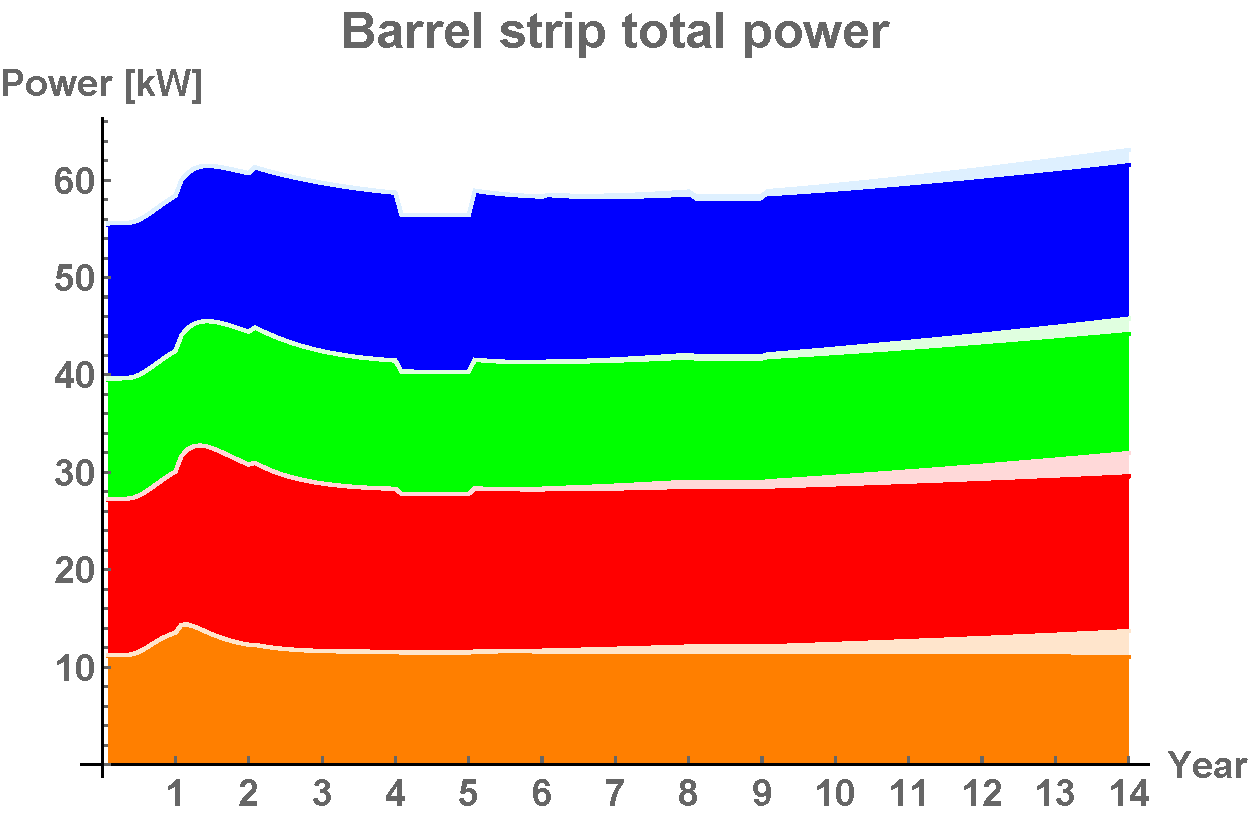
\includegraphics[width=0.45\linewidth]{figures/Totalbarrelpower-30.pdf}}\quad\quad
\subfloat[] {\label{fig:systemperformance_b} 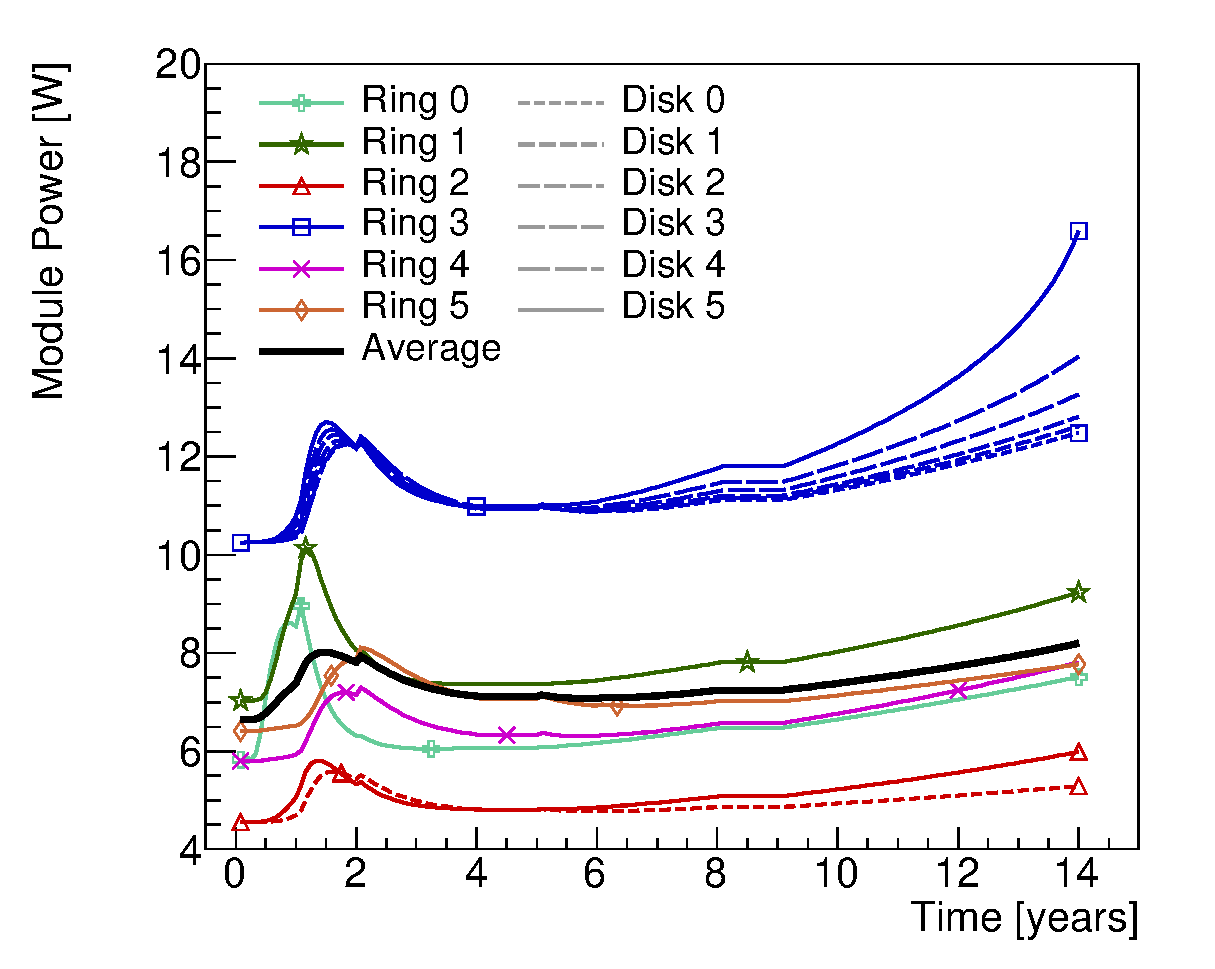
\includegraphics[width=0.45\linewidth]{figures/Endcap_ModulePower.eps}}
\caption{Examples of system performance predictions. (a) Barrel total power requirements. The plot shows the stacked power requirements for the four barrel layers (purple: layer 1, orange: layer 2, red: layer 3 blue: layer 4). Full colour indicates power from the front-end electronics, and hatched parts are contributions from HV power for the four barrels. The discontinuities in year 5 and 9 are due to anticipated year-long shutdowns of the LHC. (b) The power requirements for 12 of the 36 simulated endcap modules, labelled according to their ring type and disk position. (Modules are omitted to improve the clarity of the figure.) The solid black line indicates the average module power. Both predictions use a scenario with flat $-30^\circ$C cooling and including all safety factors.}
\label{fig:systemperformance}
\end{figure}

The predictions from this model are now used throughout the strip project to consistently size the power supply and cooling systems. Including safety factors in the predictions gives us some confidence that the designs are robust; by using commonly agreed safety factors, we ensure a consistent use of safety factors throughout the project and prevent safety factor creep.

Because of the different timescales for the peak power due to the TID effect and the radiation-induced sensor leakage, there is room to optimize the cooling temperature profile to minimize the total power in the strip system while avoiding thermal runaway. The thermo-electrical model is a powerful tool to plan such an optimized cooling profile. In fact, the cooling `ramp' scenario introduced in Section~\ref{sec:opscenarios} is the result of such an optimization.
In this scenario, depicted in Fig.~\ref{fig:rampoptimization}, the cooling temperature begins at a relatively high value ($0^\circ$~C) to minimize the impact of the TID bump in the first two years of operation, thus avoiding a peak in the module power (see Fig.~\ref{fig:rampoptimization_a}). In subsequent years, $T_C$ is steadily decreased to maintain a sensor current at or below about 1~mA, as illustrated in Fig.~\ref{fig:rampoptimization_b}, in the interest of both minimizing the module power and avoiding thermal runaway.

\begin{figure}[ht]
\centering
\subfloat[] {\label{fig:rampoptimization_a} 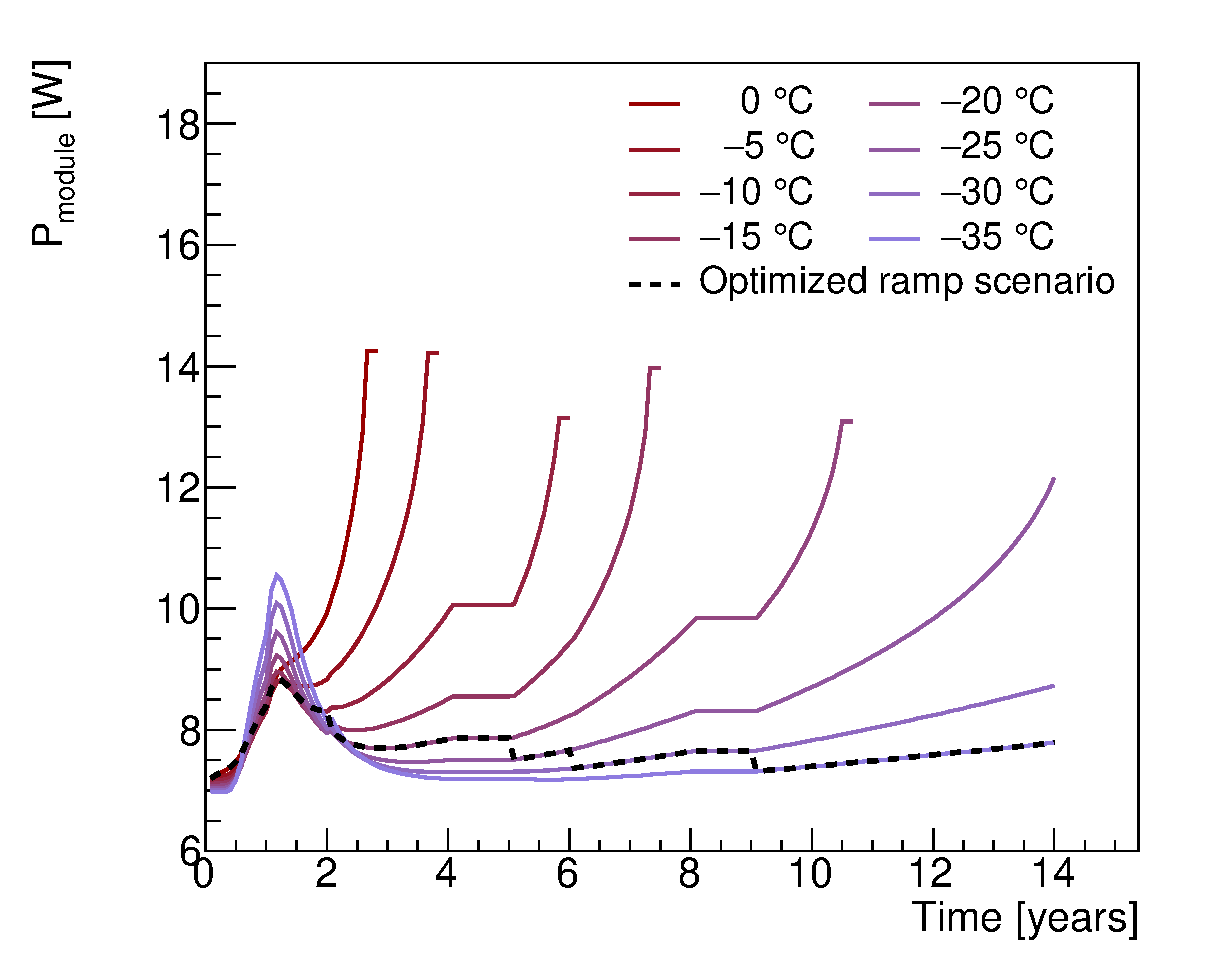
\includegraphics[width=0.45\linewidth]{figures/ModulePower_R1_newramp.eps}}\quad\quad
\subfloat[] {\label{fig:rampoptimization_b} 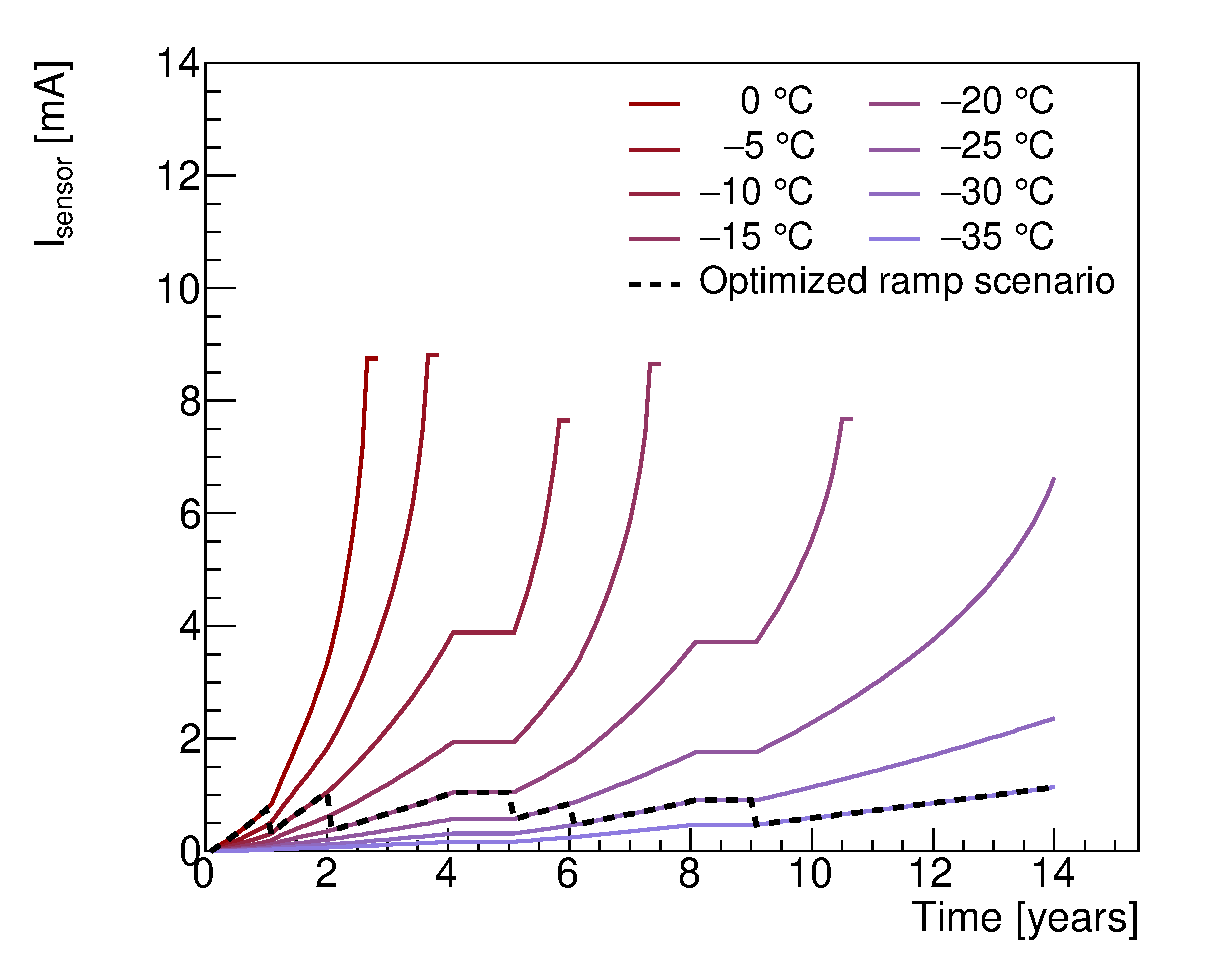
\includegraphics[width=0.45\linewidth]{figures/SensorCurrent_R1_newramp.eps}}
\caption{(a) Total power and (b) sensor leakage current of the endcap R1-type module for eight different flat cooling profiles, ranging from 0$^\circ$C to $-35^\circ$C, as well as the cooling ramp scenario specified in Fig.~\ref{fig:coolant_ramp} (dashed curve). The curves that are discontinued before year 14 correspond to scenarios that have reached thermal runaway. The cooling ramp scenario has been selected to minimize the module power while keeping the sensor leakage current stable throughout the lifetime of the ITk. All safety factors are applied in these plots.}
\label{fig:rampoptimization}
\end{figure}
